There are two major sections into which the design solution can be divided. These two sections are data and implementation. The first section, data, takes heavily from last semester's report, as there were only minor changes. 

\subsection{Data}

The data section of our design solution includes anything relevant to data, including collecting, storing, and accessing the data.
\subsubsection{Collecting Data}
Initially we had two candidates for the primary source of obtaining all NBA player and team related statistics. These two sources were: 
\begin{itemize}
\item stats.nba.com
\item basketball-reference.com
\end{itemize}
Both sources contained similar amounts of information on player matches, player season averages, teams, and matches. Basketball Reference was slightly more detailed in some aspects, such as player season averages and player matches. However, we decided to use stats.nba.com as our primary source, since we felt the official statistics platform of the NBA would have more reliable data compared to that of an unaffiliated site.

The collection of data from stats.nba.com was done by finding a webpage with pertinent data, scraping that data using Python, and storing it in a MySQL database. We automated the process of scraping the data by writing python scripts that iterate through all web pages of a specified type and searching through HTML tags to retrieve the desired data. This usually entails locating an HTML table, iterating through its rows and columns, and retrieving stats for points, assists, rebounds, etc. Two python libraries were used to build the scraper:
\begin{itemize}
\item BeautifulSoup4
\item Selenium
\end{itemize}

BeautifulSoup allows for objectification of HTML tags on a web page such that can be accessed  through python. Selenium automates the usage of a chosen browser. While, in most cases, BeautifulSoup alone would be enough to access the HTML elements of a given web page, stats.nba.com generates all of the data that we need through JavaScript. This leads to a problem, as BeautifulSoup cannot tell when a website using JavaScript has fully loaded. This is solved by using Selenium to automate browser control, as we can specify that a page is not fully loaded until all of its JavaScript components have fully loaded.


\subsubsection{Storing Data}
With respect to storing data, we considered two potential methods, each with their own advantages and drawbacks. The methods of storing data were:
\begin{itemize}
\item local database
\item remote database
\end{itemize}
The method of using a local database was enticing due to the lack of potential bottleneck associated with the connection bandwidth of a remote database. However, while examining the data on stats.nba.com, we saw that there could be the potential for needing database schema changes, as the structure was sometimes changing. In the case of a local database, this would have created an inconsistency in the local copies of each group member.

A remote database solves this issue, and also has other benefits. For one, it offers the ability to update a persistent table in parallel. In other words, multiple users can use multiple tables simultaneously to read, insert, or delete entries. Ultimately, this convenience was more beneficial than the cost of overhead in access time to a remote database.

\subsubsection{Accessing Data}
Each group member was given credentials with which he/she could access the remote database through SSH. This was possible from any location with internet access.

\subsection{Implementation}
We began designing the software architecture before finishing the aforementioned database design. Our initial design was a single NN that took in, as input, all of the stats of every active NBA player. Additionally, it had an extra input for every player which was set to 1 if the player was playing tonight, and 0 if the player was not.  These were called the ``who's playing indicators''. The output of this NN was the best lineup for the competition. A block diagram of this system can be seen in Figure \ref{fig:first_iteration}.
\begin{figure}[ht]
    \centering
    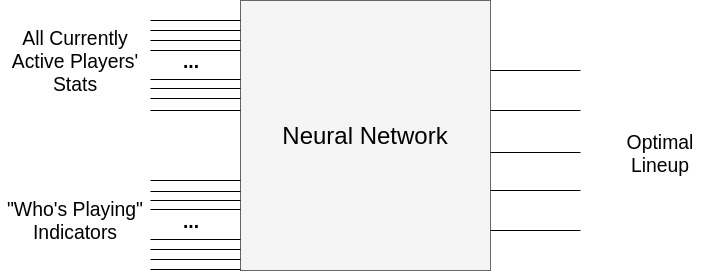
\includegraphics[width=0.75\textwidth]{figures/first_iteration}
    \caption{First design iteration}
    \label{fig:first_iteration}
\end{figure}
 
After discussing this design within our group and with our supervisor, we realized it had major limitations, listed below. First, this system would only use data from active players. This was not taking advantage of the many decades of basketball data to which we had access. Second, it would also require a massive amount of data to be able to learn properly. This is because, generally, the amount of data required to learn adequately is correlated with both the complexity, and the number of, inputs. %TODO citation
Third, there would be many unused inputs each time the system is used. Since there are usually around six NBA games each night, there are 120 active players on a single night. There are about 500 total active players, which means that there would be about 380 unused inputs. Although this is not explicitly a problem, it makes it seem like there would be a better way to structure the design. The final limitation of the initial NN design was that it would be prone to discover imaginary correlations. 
%WEAK%
Since the NN only knows which players are playing, and not on which team, it would be bound to find correlations between players that are not playing against each other. To explain, if Team A is playing against Team B in one game, and Team X is playing against Team Y in another, the NN may find a relationship between players on Team A and on Team B. This is despite the fact that they are not playing against each other, and that these games are independent.\\
%WEAK%
Taking these limitations into account, we designed an improved architecture that was more flexible and required less data to train. We decided on a three step system, of which only one part would involve machine learning. The first system was used to calculate players' scores, the second system used these as inputs to predict player game scores, and the third system selected optimal lineups. An overview of this software architecture can be seen in Figure \ref{fig:second_iteration}.
\begin{figure}[ht]
    \centering
    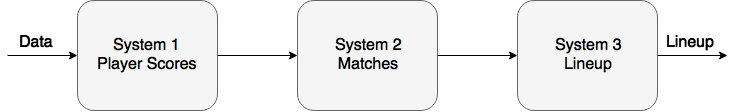
\includegraphics[width=0.85\textwidth]{figures/second_iteration}
    \caption{Redesigned System Architecture}
    \label{fig:second_iteration}
\end{figure}

These three systems will now be looked at in detail.

\paragraph{System 1: Calculating Player Scores}\mbox{}\\
The first step of the design solution was to calculate a score for each player who has played in the NBA. This score is a representation of how good the player is at scoring fantasy points "in a vacuum". That is to say, how well a player will perform with respect to the fantasy system, if we ignore the match-specific variables, namely who is on his team and who he is playing against. Calculating the most accurate score to represent this is not an exact science. The most straightforward solution was to use the same points system as FanDuel for calculating fantasy points. Since we wanted to spend more time focusing on the second system (NN), we opted for this simple equation, the details of which can be seen in Figure \ref{fig:comp_lineup}. Due to the modularity of the code, this score can be easily changed and validated on, and ways to do that will be discussed in future plans. With this formula, we calculated two different types of this score for each player: a short term score, and a long term score. The short term score used the player's average statistics of the last n (chosen as 5) games. The long term score used the player's average statistics of their previous season. In the case where it was a player's first season, it took his current season's statistics so far as input.
\begin{figure}[ht]
    \centering
    \includegraphics[width=0.5\textwidth]{figures/player_scores}
    \caption{Player scores system}
    \label{fig:player_scores}
\end{figure}
%TODO fix this graphic (it isn't right)
\paragraph{System 2: Matches Neural Network}\mbox{}\\
The scores for every player, obtained in the first step, are then used as inputs for the matches NN. The matches neural net puts two teams of players, each represented by two scores, "against each other". That is to say, the first fourteen inputs are used for seven of Team A's players (short term and long term score each), and the next fourteen are used for seven of Team B's players. We selected seven as a compromise between being too restrictive (not all teams have many active players in each position), and not having enough inputs. The players on each team are ordered by their basketball position. The basketball positions given by our source are guard (G), forward (F), and center (C). As not each team plays the same amount of players in each position, we had to determine what a representative combination of the above positions would look like, which will be discussed in the Data Results section. Ultimately, we decided that a representative set for which we had data would be one center, three guards, and three forwards.\\
The output of the NN is a ``fantasy game score'' for each player. The benefit of this NN is that, since all basketball matches follow the same rules, with the most impactful variable being the skill level of each player on either team, we can train this net on every match that has happened in the past 50 years, and still use it to predict scores for matches today. A point guard in 1980 who had incoming scores of [10, 10] will be treated the same as a point guard today with those scores. This NN has a relatively low amount of inputs, none of which are unused. This means it needs less data to train successfully. This design can be seen in Figure \ref{fig:neural_network_full}.

\begin{figure}[ht]
    \centering
    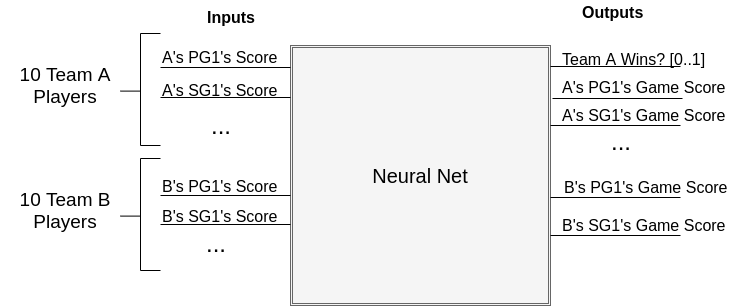
\includegraphics[width=0.6\textwidth]{figures/neural_network_full}
    \caption{Desired complete matches neural network}
    \label{fig:neural_network_full}
\end{figure}

Initially, this network was set to only predict the team that won or lost, and not the game scores of the players. This first prototype was thus not applicable for fantasy basketball, but was used to become familiar with TensorFlow and best practices. We experimented with different input features to see how they impacted the accuracy of the network. In the end, with these ordered positions, the network reached a 63\% prediction accuracy. %TODO Figure here of first sys
We did not spend much time attempting to increase this value, as it was an aside from our main goal, predicting lineups.


\paragraph{System 3: Choosing Lineups}\mbox{}\\
The choosing lineups system takes as input the player game scores, salaries, positions of each player in tonight's games, as well as the total budget we are working with, and outputs lineups with maximized summed player scores. This problem was similar to a backpack problem, but with more constraints. We selected the python library PuLP as the tool to use to solve this constraint problem, and found it to be quite effective. As well, we were able to use this system to generate multiple lineups by applying Gaussian noise to the players' scores before passing these to the system.
%TODO stephen write here about detailed implementation. need figure.
The objective function we sought to maximize had the following structure:

\[ z = p_1*x_1 + p_2*x_2 + ... + p_n*x_n \]

In this, \textit{z} is the objective function, \textit{n} is the number of players we have on a given night, each \textit{p} variable represents one of the \textit{n} players, and each \textit{x} variable is a binary decision variable that will indicate whether or not the corresponding player has been chosen or not.

Maximizing the objective function was subject to six constraints. The first five constraints specified the number of players of each position type we were allowed to have in our lineup. Specifically, the constraints of our fantasy league require our lineup to have exactly two point guards, two shooting guards, two small forwards, two power forwards, and one center. The constraint specifying the number of allowed point guards, for example, looked like this:

\[ x_1 + ... + x_j = 2 \]

where \textit{x\textsubscript{1}} to \textit{x\textsubscript{j}} are the binary decision variables of the point guards playing on a given night. The remaining four positional constraints are structured in the same way.

The final constraint ensures that we respect the total budget we are working with when purchasing players. It simply says that the the sum of the costs of the players selected cannot exceed the total budget we have to work with. This is shown in the equation below:

\[ p_1*x_1 + p_2*x_2 + ... + p_n*x_n <= Total Budget \]

As was the case in the objective function, \textit{n} is the number of players we have on a given night, each \textit{p} variable represents one of the \textit{n} players, and each \textit{x} variable is the binary decision variable for the corresponding player.

Although there exist several ways of solving integer linear programming programs, the python PuLP library handles this decision for us. Inputting the objective function and constraints mentioned above is sufficient for PuLP to find an optimal lineup solution.

\paragraph{Cross Validation \& Testing}\mbox{}\\
In order to properly test this system, we needed to define a success metric, or a way of measuring how well the system was performing. Ideally, this metric would be profitability, but this was not possible without the historic competition data. Instead, we used a heuristic which is given in Equation \ref{eq_heuristic}

\begin{equation}
Performance = \frac{Maximum Theoretical Lineup Score}{Actual Score of Predicted Lineup}
\label{eq_heuristic}
\end{equation}

This formula yielded around 60\% with random choices between the top seven players on each team. In order to determine what percentage needed to be reached to be profitable, we examined current competitions, and found an effective rule. A system was profitable in most of these competitions when this performance metric reached 80\%, i.e. when the score reached 80\% of the maximum theoretical score. Figure \ref{fig:80pRule} shows this relationship, where the last winning score is roughly 79\% of the maximum.
\begin{figure}[ht]
    \centering
    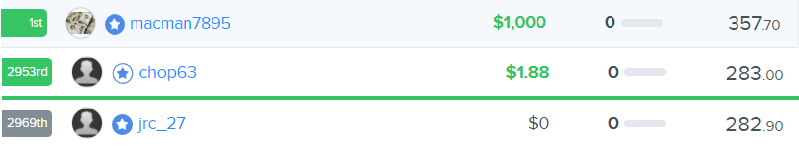
\includegraphics[width=0.6\textwidth]{figures/winningvslosing}
    \caption{Scores for best lineup and barely profitable lineup}
    \label{fig:80pRule}
\end{figure}
In order to increase our performance, we began to train the network. In doing so, we realized that one of the limitations of training and attempting to cross-validate the hyperparameters was the computational time. To remedy this, we rented a remote computer with a powerful GPU, %TODO what GPU?
 and changed our machine learning code to be GPU optimized by switching from TensorFlow to TensorFlowGPU. %TODO check this with Flo
The service we used was called Paperspace, and it was chosen for its low hourly rates with no commitment requirement. We ran cross-validation on Paperspace, and were able to increase our performance metric to 82\% - just above the profitability line. Thus, we began testing in actual competitions; the results of doing so will be discussed in the implementation results section.

\subsection{Results and Discussion}
There are two types of results that will be given in this report. The first are those related to how much data was scraped from our source, or generated, and the second is related to the success rate of the neural network.

\subsubsection{Data Results}
We managed to scrape, collect, and otherwise compute a significant amount of data to be stored in our database. We were able to gather all data for every basketball game since 1979. We have data for 42000 matches, 10000 player-seasons (unique players for a specific season), 2000 players, and 36 teams, including some that are no longer active. For each match, there are about 15 players with statistics for that match. This is entered in our "player matches" table, and we currently have data in this table for about 25\% of matches. This corresponds to 250,000 entries, and yields about 13000 inputs for our neural net. However, the different architectures which have been presented all impose different constraints on the inputs themselves. For example, the neural network with ordered player scores shown in Figure \ref{fig:neural_network_ordered} requires the match input to have both teams with at least the minimum number of  players (7 in this instance). The neural net with players ordered by position has even more constraints. Not only does it require a minimum number of players per team, but also it needs a minimum number of players per \textit{position}. When performing an analysis on the different player positions per lineup, we found significant variation between teams. This was complicated even further as some players played multiple positions, denoted by two positions separated by a hyphen. For example, the position "F-G" meant that the player could either play a forward or a guard. We found 21 possible combinations of these positions that teams could play. As an example, playing "C, G, G, F, F, C-F" could be a single combination, whereas "F-G, C, C-F, F, F, G, G" could be another. We found that none of the possible 21 combinations had enough data to train our neural network on. Even our initially designed input format of requiring two guards, one center, and two forwards per team (meaning only five inputs per team) caused roughly 21\% of inputs to be discarded, simply because these inputs did not meet the criteria of having these specific numbers of players in each positions.

To avoid losing significant amounts of input data due to constraints, we simplified our input scheme by combining the multi-position players with the single-position players. Our methods of combining these players is shown in Figure \ref{fig:distributionAfterCombination}. Note that the first combination has zero centers (hence no blue bar). In using this scheme, we were able to reduce the amount of lost data to a mere 11\%.

\begin{figure}[ht]
    \centering
    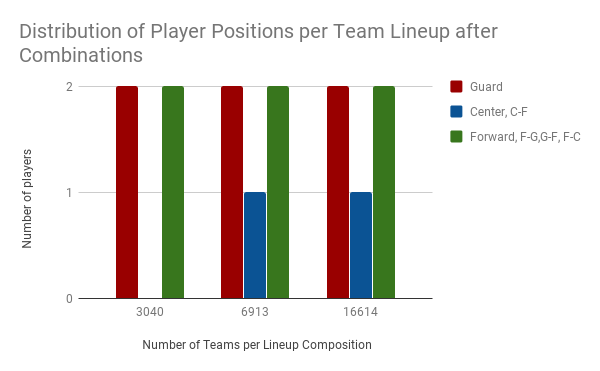
\includegraphics[width=0.75\textwidth]{figures/distributionAfterCombination}
    \caption{Team Compositions by Player Positions After Combinations}
    \label{fig:distributionAfterCombination}
\end{figure}

\subsubsection{Implementation Results}
As mentioned in the description of the NN in the implementation section, we tested many different system architectures. The final three-system architecture will be the only one discussed in this section, as it is the only one used to enter real competitions. For the results of the earlier architectures, please see our report from the previous term.

Note that the provided results results are on the cross-validated version of the neural network, with two hidden layers, 128 hidden nodes per layer, and a learning rate of 0.01. Furthermore, all accuracy results were obtained by using 70\% of the input data to train the network, and 30\% to test.\\

%TODO Flo to add meaningful data here
\textit{Under construction: we will add data on training/cross-validating here}

After cross-validating the system, and entering the first lineups into competitions, we realized we had overlooked some potential issues. First, the database was not updated, meaning that the short-term scores of each player were actually scores from months ago. Second, we found that we were accidentally ignoring one or two games per night, due to a bug with the positional constraints in our code. Thus, our output was only predicting a lineup on a subset of the games each night. Third and finally, we found that many of our selected players did not end up playing each night, yielding zero points. This third issue proved the most challenging to tackle. Although we checked for injuries, we did not perform a more thorough check than this. Initially, we hoped that we could solve this with more checks in our code, but we quickly learned that this was not feasible. Ultimately, before submitting each lineup, it is an important step for the user to read recent news about the NBA player. Sometimes players do not play for personal issues, or because they were only temporarily playing in the spot of another player. This is both difficult and unnecessary to try to predict. Instead, we added an option for our system to ignore certain players, entered manually.

After solving these issues, we continued entering competitions. To our surprise, the system was successful. Figure \ref{fig:win_record} shows a brief summary of each competition we participated in where all of our players played.
\begin{figure}[ht]
    \centering
    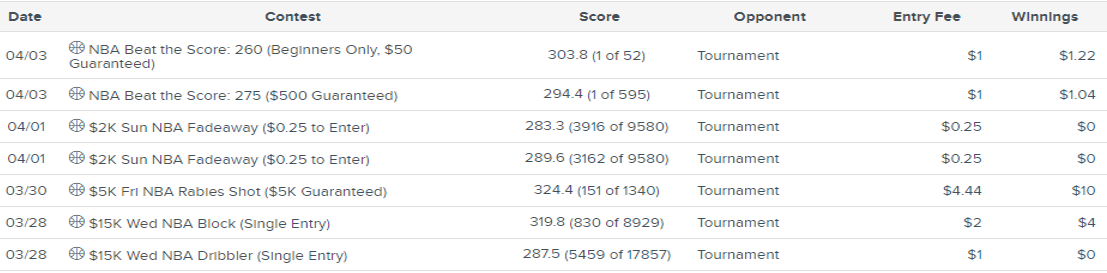
\includegraphics[width=0.6\textwidth]{figures/fanduel_comp}
    \caption{Competition record for submitted lineups}
    \label{fig:win_record}
\end{figure}
One can see that we are overall profitable, but not reliably so, and on a small sample size. When examining the lineups in detail, one can make some interesting observations. For instance, sometimes the network was able to make good predictions that were missed by other competitors. For each player selected, at the end of the competition, a value is given that shows what percentage of other competitors also selected that player. In our best lineup, our players were picked on average 7.5\% by others. By contrast, the nearest competitor's players averaged a 27\% pickrate. Our lineup containing these picks can be seen in Figure \ref{fig:good_picks}. Note that a typical score value for a player with a \$5000 salary is about 15.

\begin{figure}[ht]
    \centering
    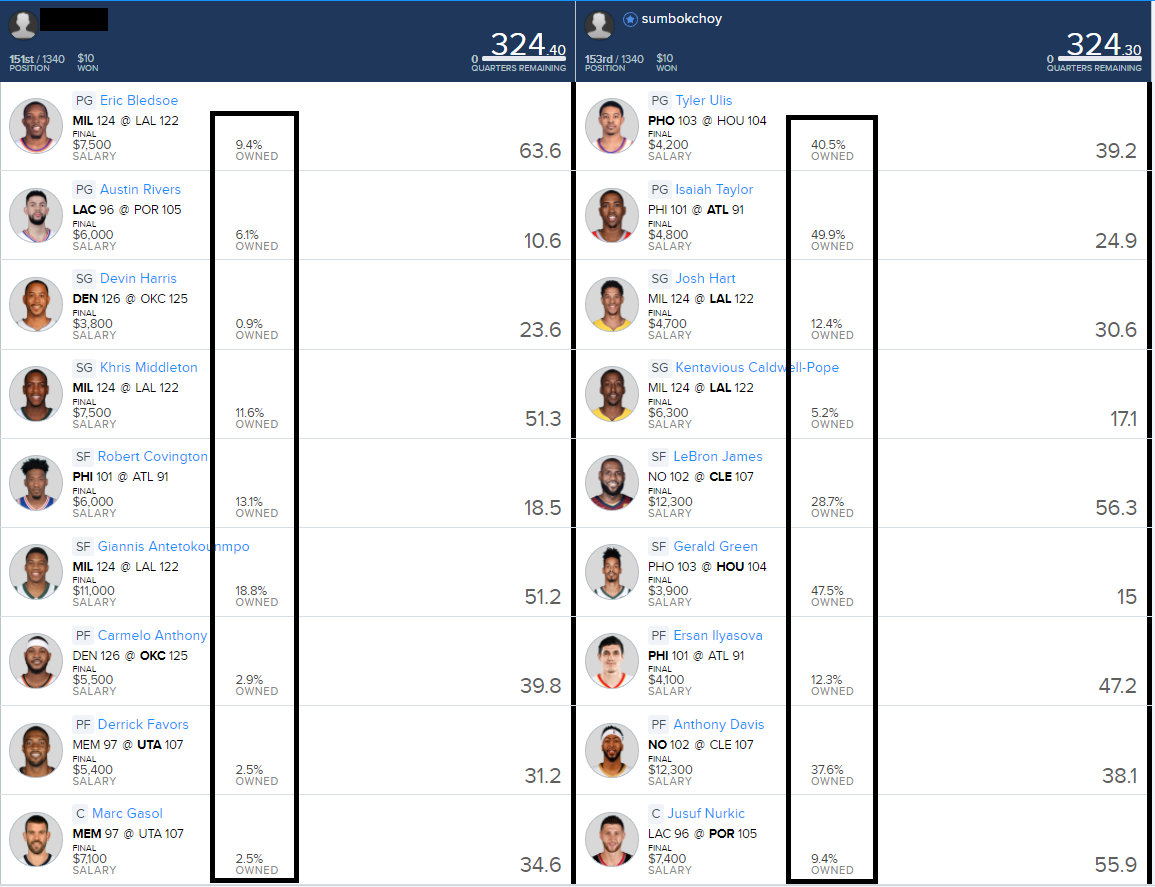
\includegraphics[width=0.8\textwidth]{figures/mevsbest}
    \caption{Good rare picks of our system versus those of a near competitor}
    \label{fig:win_record}
\end{figure}

 %TODO highlight the players right here.
This supports our hypothesis that our system would be able to make good predictions that were missed by others, thus giving it the potential to perform quite well in top-heavy competitions.

It is also worth noting that, even in the competitions that the system does not succeed, it is still performing above average, always in the top 50th percentile. This is especially remarkable since almost all of the other competitors are marked as experienced. Figure \ref{fig:competitors} shows a sample of the winning and losing players for a competition, including their experience emblems.
\begin{figure}[ht]
    \centering
    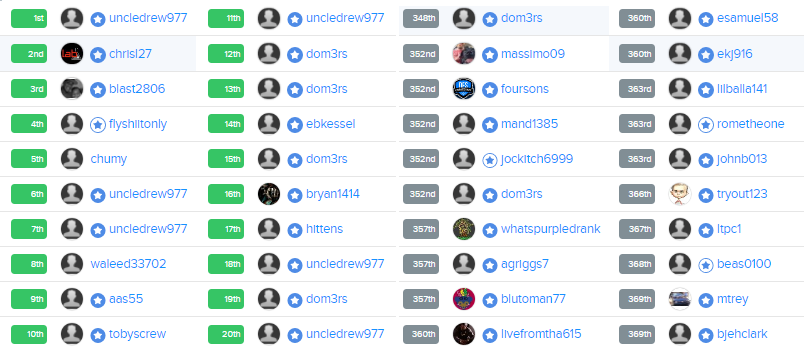
\includegraphics[width=0.6\textwidth]{figures/competitors}
    \caption{Experience level of competitors}
    \label{fig:competitors}
\end{figure}
Competitors with a white star and blue circle have been in over 1000 competitions and have won at least \$1000 across four contests whereas competitors with a blue star and white circle have been in at least 500 competitions or have won at least \$1000 across four contests. We measured the percentage of experienced players for a single competition, and found it to be 85\%. Our system was able to perform quite well against these experienced players, turning a profit in lineups that had all players active. However, the system is still far from being reliably profitable, as its outputs are high in variance. There are still improvements to be made.

